%%%%%%%%%%%%%%%%%%%%%%%%%%%%%%%%%%%%%%%%%%%%%%%%%%%%%%%%%%%%%%%%%%%%%%%%%%%%%%%%
% AMS Beamer series / Bologna FC / Template
% Andrea Omicini
% Alma Mater Studiorum - Università di Bologna
% mailto:andrea.omicini@unibo.it
%%%%%%%%%%%%%%%%%%%%%%%%%%%%%%%%%%%%%%%%%%%%%%%%%%%%%%%%%%%%%%%%%%%%%%%%%%%%%%%%
%\documentclass[handout]{beamer}\mode<handout>{\usetheme{default}}
%
\documentclass[presentation, 10pt,aspectratio=169]{beamer}\mode<presentation>{\usetheme{AMSBolognaFC}}
%\documentclass[handout]{beamer}\mode<handout>{\usetheme{AMSBolognaFC}}
%%%%%%%%%%%%%%%%%%%%%%%%%%%%%%%%%%%%%%%%%%%%%%%%%%%%%%%%%%%%%%%%%%%%%%%%%%%%%%%%
\usetheme{metropolis}
  
\usepackage{lmodern}
\usepackage{fontawesome}
\usepackage[sfdefault]{FiraSans} %% option 'sfdefault' activates Fira Sans as the default text font
\usepackage[T1]{fontenc}
\renewcommand*\oldstylenums[1]{{\firaoldstyle #1}}
\usepackage{arev}
\usepackage{multicol}
\usepackage{wasysym}
\usepackage{amsmath,blkarray}
\usepackage{centernot}
\usepackage{fontawesome}
\usepackage{fancyvrb}
\usepackage[ddmmyyyy]{datetime}
\renewcommand{\dateseparator}{}
%\renewcommand{\thefootnote}{\fnsymbol{footnote}}
\newcommand{\version}{1}
\usepackage{biblatex}
	\makeatletter

% #FAFAFA
\definecolor{customfg}{RGB}{250, 250, 250} % White
% #23373B
\definecolor{custombg}{RGB}{35, 55, 59} % Dark Blue
\addbibresource{biblio.bib}
%%%%%%%%%%%%%%%%%%%%%%%%%%%%%%%%%%%%%%%%%%%%%%%%%%%%%%%%%%%%%%%%%%%%%%%%%%%%%%%%
\title[Il Potenziale dell'Intelligenza Artificiale Collettiva]
{Oltre l'IA Individuale: }
%
\subtitle[Il Potenziale dell'Intelligenza Artificiale Collettiva]
{Il Potenziale dell'Intelligenza Artificiale Collettiva}
%
\author[Aguzzi]
{\textbf{Gianluca Aguzzi} \href{mailto:gianluca.aguzzi@unibo.it}{gianluca.aguzzi@unibo.it}}
%
\institute[DISI, Univ.\ Bologna]
{Dipartimento di Informatica -- Scienza e Ingegneria (DISI)\\\textsc{Alma Mater Studiorum} -- Universit{\`a} di Bologna}
%
\renewcommand{\dateseparator}{/}
\date[\today]{\today}
%
%%%%%%%%%%%%%%%%%%%%%%%%%%%%%%%%%%%%%%%%%%%%%%%%%%%%%%%%%%%%%%%%%%%%%%%%%%%%%%%%ù
\metroset{block=fill}
\begin{document}

\nocite{*}
\frame{\titlepage}

{
\setbeamercolor{background canvas}{bg=custombg} % Set background to foreground color
\setbeamercolor{normal text}{fg=customfg}    

\begin{frame}[c]
	
	{
	\color{customfg}
	\begin{center}
	\Large\textbf{Hello World! \faSmileO}

	\begin{tikzpicture}
		\clip (0,0) circle (1.5cm) node {\includegraphics[width=3cm]{img/me-3.jpeg}};
	\end{tikzpicture}
	\color{customfg}{
	\small
	\begin{itemize}
		\color{customfg}
				\item \alert{\faGraduationCap} ~ \textbf{Dottorato} in Ingegneria e Scienze Informatiche (2024)
				\item \alert{\faPencilSquare} ~ \textbf{Professore a contratto} @ Università di Bologna (campus di Cesena)
				\item \alert{\faFlask} ~ \textbf{Background}: Ingegneria del Software (Sviluppatore Scala) \& Apprendimento Automatico (Apprendimento per Rinforzo) \& Pensiero Computazionale
				\item \alert{\faSearch} ~ \textbf{Interessi di Ricerca}: Intelligenza Collettiva, Apprendimento per Rinforzo Multi-Agente
			\end{itemize}
	}
	\end{center}
}
\end{frame}
}

\begin{frame}{Outline}
	\begin{itemize}
		\item Oggi parleremo d'\alert{\textbf{Intelligenza Collettiva}} e \alert{\textbf{Sistemi Collettivi Adattativi}}, focalizzandoci su
		\begin{itemize}
			\item Cosa sono i sistemi collettivi adattativi e come si differenziano da altri sistemi
			\item Come si progettano sistemi che mostrano \underline{intelligenza collettiva}
			\begin{itemize}
				\item \emph{Approcci manuali} (ispirati biologia, programmazione aggregata)
				\item \emph{Approcci automatici} (algoritmi genetici, apprendimento per rinforzo multi-agente)
			\end{itemize}
			\item Direzioni di ricerca
			\begin{itemize}
				\item \emph{Approcci ibridi}
				\item Modelli \underline{fondazionali} per l'intelligenza collettiva
			\end{itemize}
			Ma prima, un po' di contesto \alert{\faSmileO}
		\end{itemize}
	\end{itemize}
\end{frame}

\section{Contesto - Sistemi Collettivi Adattativi}
%% change the background image
{
\usebackgroundtemplate%
{\includegraphics[width=\paperwidth,height=\paperheight]{img/frame-1.png}}
\begin{frame}\end{frame}
}
{
\usebackgroundtemplate%
{\includegraphics[width=\paperwidth,height=\paperheight]{img/frame-2.png}}
\begin{frame}\end{frame}
}
{
\usebackgroundtemplate%
{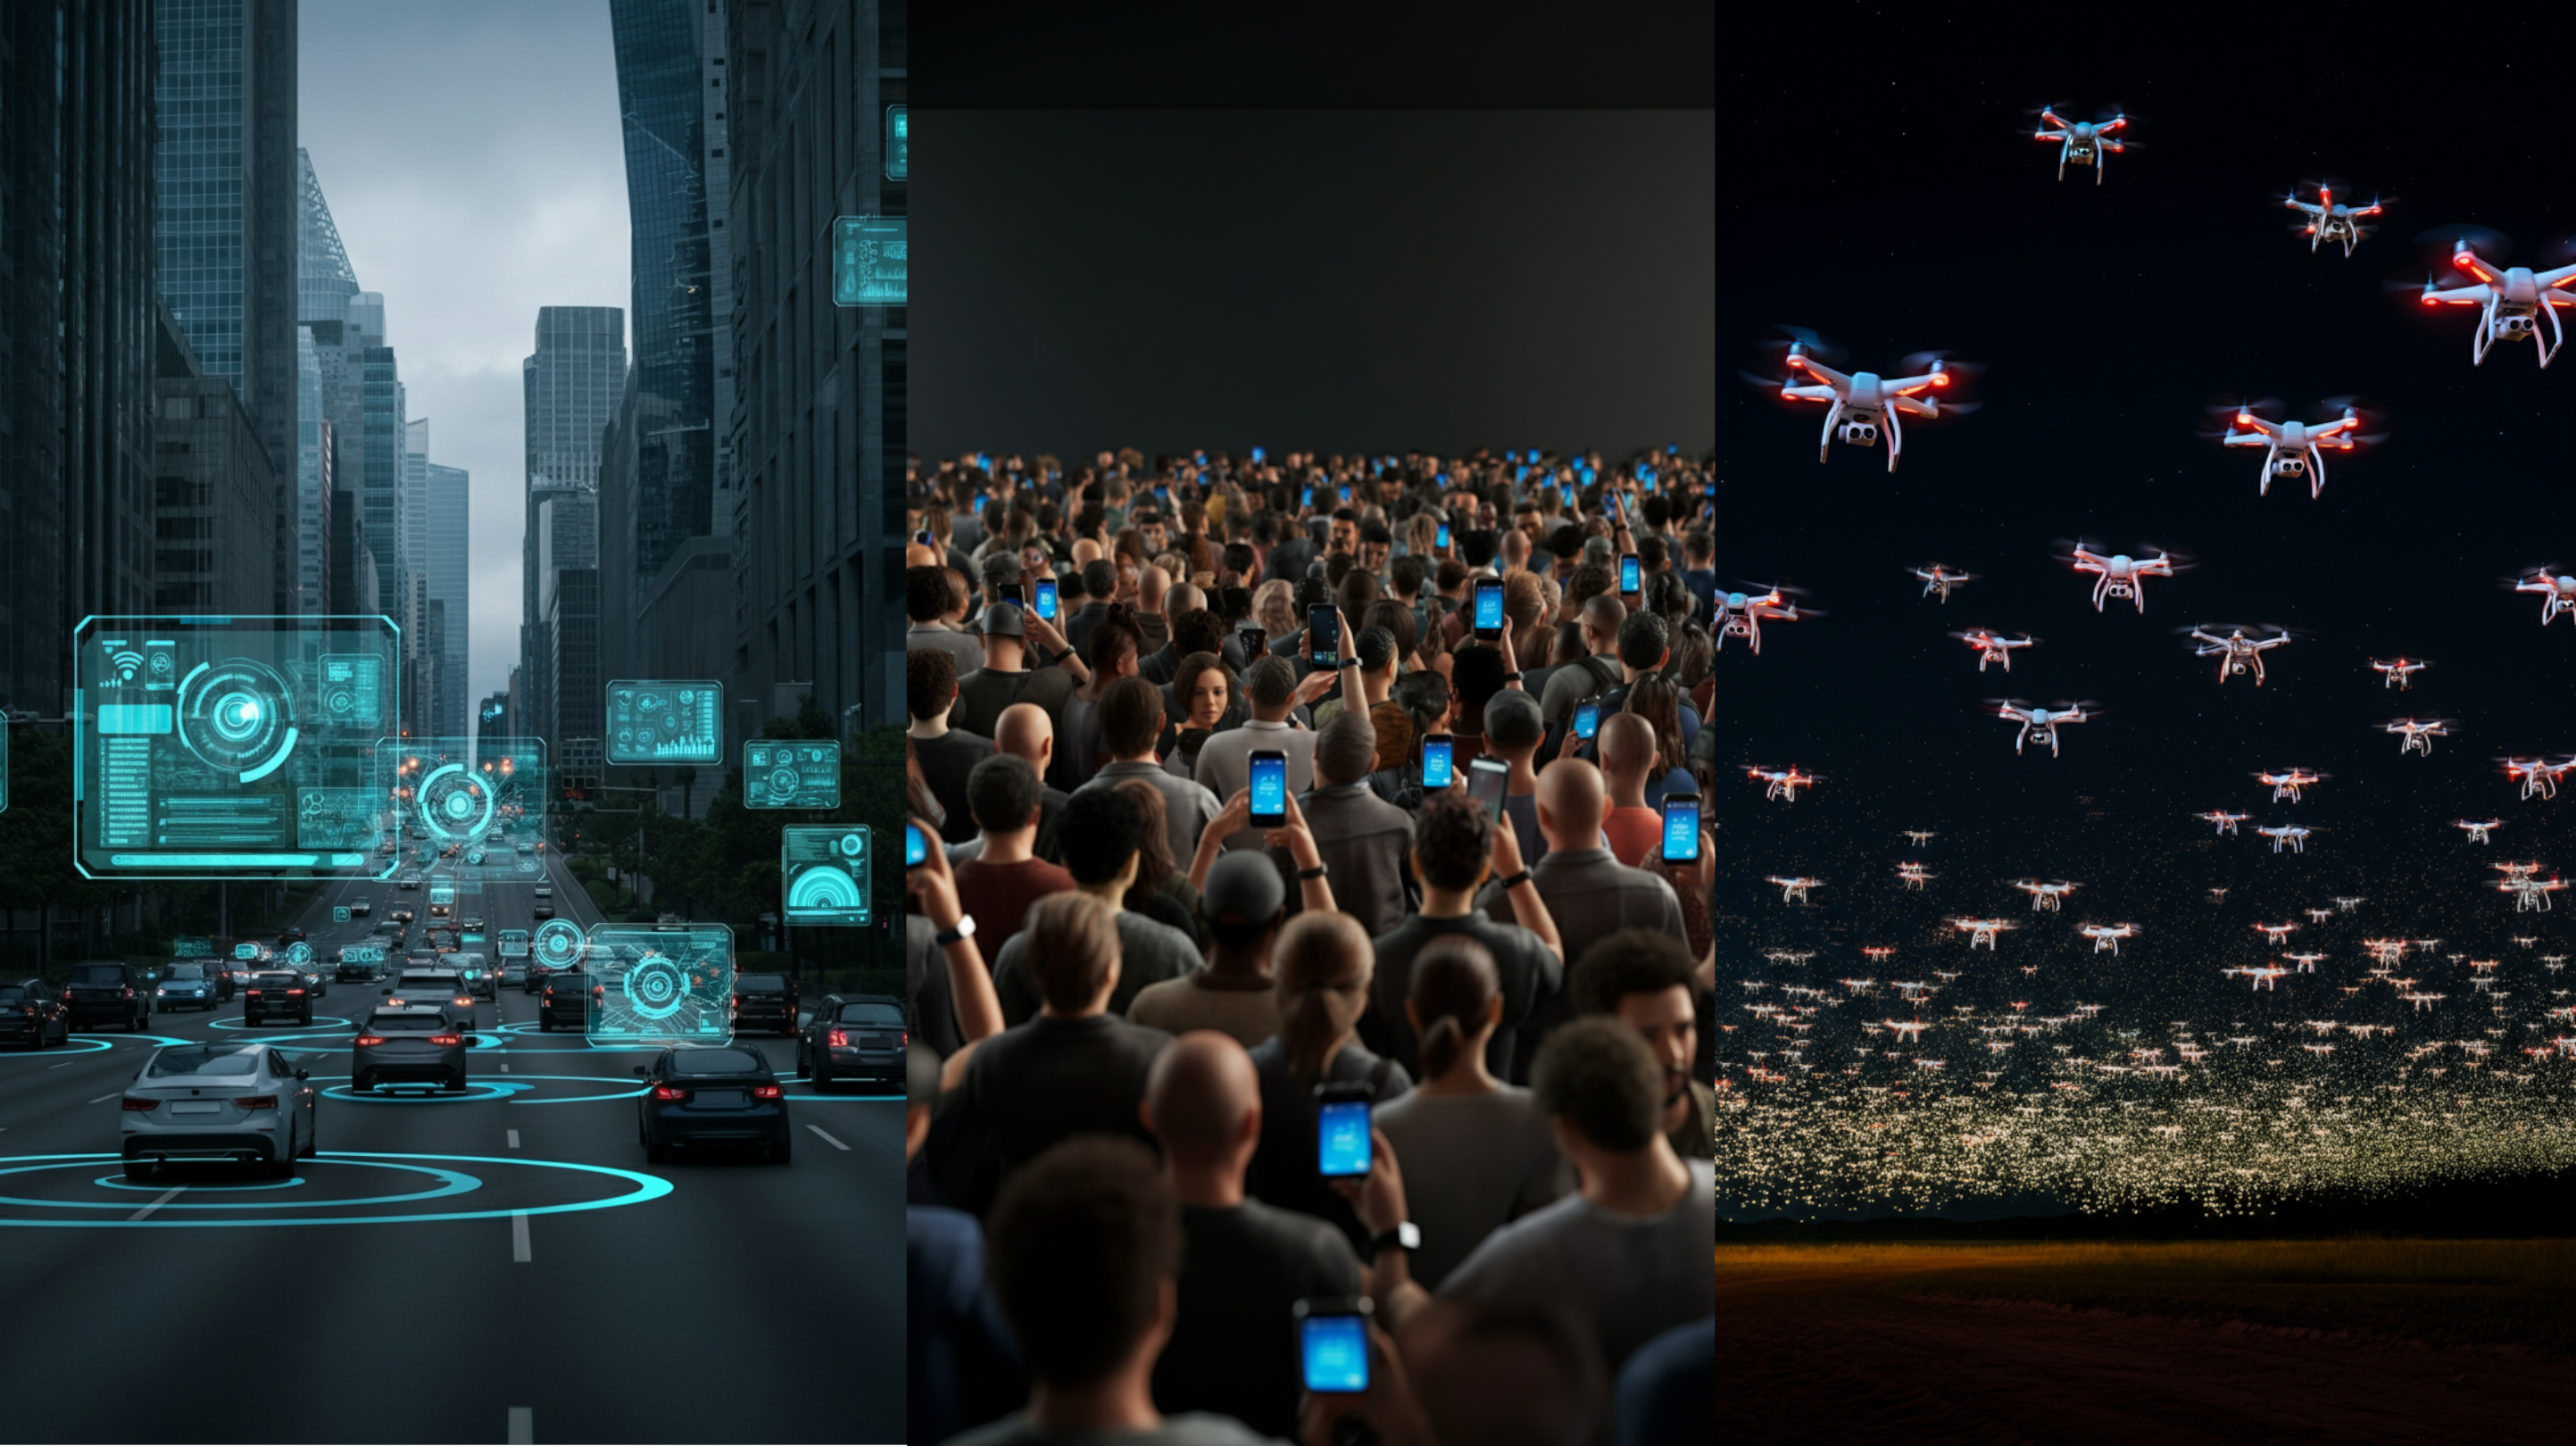
\includegraphics[width=\paperwidth,height=\paperheight]{img/frame-3.png}}
\begin{frame}\end{frame}
}
\begin{frame}{Panorama Computazionale Moderno}
	\begin{itemize}
		\item Centinaia/Migliaia di dispositivi computazionali
		\item Altamente eterogenei e distribuiti
		\item Interconnessi tramite reti di comunicazione
		\begin{itemize}
			\item \textbf{Internet of Things} (IoT)
		\end{itemize}
		\item Applicazioni \alert{\emph{situate}} e \alert{\emph{ubiquite}}
		\begin{itemize}
			\item Context-aware
			\item Pervasiveness (la computazione che ``scompare'')
		\end{itemize}
		\item L'umano è parte integrante del sistema
		\begin{itemize}
			\item Human-in-the-loop
		\end{itemize}
		\item \alert{\textbf{Come possiamo progettare sistemi artificiali che si adattano a questo contesto?}}
		\item \alert{\faLeaf} ~ Inspiriamoci a come la natura affronta problemi simili ~ \alert{\faLeaf}
	\end{itemize}
\end{frame}
\begin{frame}[fragile]{Animali Sociali}
% https://cric96.github.io/hello-aarhus/#/3/5/3
\begin{center}
	\href{https://youtu.be/IpKL-URul2I}{\includegraphics[height=3.7cm]{img/example.png}}
	\href{https://www.youtube.com/watch?v=ZGvtnE1Wy6U&t=37s}{\includegraphics[height=3.7cm]{img/fireflies.png}}
	\href{https://youtu.be/B6M_XgiONoo}{\includegraphics[height=3.7cm]{img/school.png}}
\end{center}
In tutti questi scenari, gli animali/organismi mostrano una sorta di \underline{\alert{\textbf{intelligenza collettiva}}}.
\end{frame}
{

\setbeamercolor{background canvas}{bg=custombg} % Set background to foreground color
\setbeamercolor{normal text}{fg=customfg}    

\begin{frame}[c]
	
	{
	\color{customfg}

	\begin{center}
	\Large\textbf{Intelligenza Collettiva} \emph{Artificiale} \\
	
	L'\alert{\emph{intelligenza}} che può essere attribuita a un \alert{\emph{collettivo}}.
	\\ \vspace{1cm}
		\large{\alert{Intelligenza}} \faArrowRight ~ Misura la capacità di un agente di raggiungere \underline{\emph{obiettivi}} in un'ampia gamma di ambienti.  \\

		\large{\alert{Collettivo}} \faArrowRight ~ Gruppi d'individui (membri) che manifestano una qualche forma di \underline{\emph{unità}}. \\

	\end{center}

	\vspace{1cm}	
}
\end{frame}
}
\begin{frame}{Intelligenza Collettiva E Sistemi Collettivi Adattativi}
	\begin{alertblock}{Definizioni -- Cont.}
		\begin{itemize}
			\item \emph{Gruppi d'individui che agiscono collettivamente in modi che sembrano intelligenti.} -- focus sul concetto di \alert{gruppo}
			\item \emph{Intelligenza che emerge a livello macro di un collettivo e trascende quella dei singoli individui.} -- focus sul livello \alert{macro} e \alert{micro}
		\end{itemize}
	\end{alertblock}
	\begin{exampleblock}{Sottoclassi di Intellingenza Collettiva}
		\begin{itemize}
			\item Intelligenza di \emph{Sciame} (\alert{Swarm Intelligence}): Intelligenza collettiva osservata in gruppi di \emph{animali}
			\item Intelligenza di Folle (\alert{Crowd Intellingece}): Intelligenza collettiva osservata in gruppi di \emph {persone}
		\end{itemize}
	\end{exampleblock}
	\begin{block}{Sistemi Collettivi Adattativi (CAS)}
		Sistemi composti da un insieme di agenti autonomi che mostrano intelligenza collettiva.
	\end{block}
\end{frame}
\begin{frame}{Collective Adaptive System}
\begin{alertblock}{Caratteristiche (tratte dagli animali sociali)}
	\begin{itemize}
		\item \textbf{Decentralizzazione} \faArrowRight ~ Nessun controllo centrale
		\item \textbf{Adattabilità} \faArrowRight ~ Capacità di adattarsi a cambiamenti ambientali
		\item \textbf{Scalabilità} \faArrowRight ~ Capacità di crescere in numero d'individui 
		\item \textbf{Emergenza} \faArrowRight ~ Comportamenti collettivi che emergono da interazioni locali
		\item \textbf{Robustezza} \faArrowRight ~ Capacità di sopportare guasti
	\end{itemize}	
\end{alertblock}

\begin{exampleblock}{Sfide ingegneristiche}
	\begin{itemize}
		\item \textbf{Fallimenti} \faArrowRight ~ I fallimenti sono così comuni che diventano parte del design
		\item \textbf{Mapping tra micro e macro} \faArrowRight ~ Come i comportamenti locali dei singoli agenti si traducono nei comportamenti collettivi?
		\item \textbf{Unknown unknowns} \faArrowRight ~ Come progettare sistemi che si adattano a situazioni non previste?
	\end{itemize}
\end{exampleblock}
\end{frame}
\begin{frame}{Progettare Sistemi Collettivi Adattativi}
	\begin{itemize}
		\item \textbf{Approcci manuali} \faArrowRight ~ Programmazione ispirata a (o basata su) sistemi biologici:
		\begin{itemize}
			\item \alert{Bottom-up} \faArrowRight ~ Si imita la natura per progettare sistemi collettivi adattativi
			\item \alert{Top-down} \faArrowRight ~ Ispirandosi ai meccanismi biologici, si introducono nuove \emph{astrazioni} per progettare sistemi collettivi adattativi
			\begin{itemize}
				\item \textbf{Macro programmazione} \faArrowRight ~ Linguaggi di programmazione che inseriscono il collettivo come \underline{entità di prima classe}
			\end{itemize}
		\end{itemize}
		\item \textbf{Approcci automatici} \faArrowRight ~ Progettazione di sistemi collettivi adattativi tramite algoritmi automatici
		\begin{itemize}
			\item \alert{Algoritmi Genetici} \faArrowRight ~ Evoluzione di popolazioni di agenti
			\item \textbf{Apprendimento per Rinforzo Multi-Agente} \faArrowRight ~ Apprendimento per rinforzo in sistemi multi-agente
		\end{itemize}
	\end{itemize}

	È cruciale sfruttare le \alert{\textbf{simulazioni}} per testare le ipotesi e validare i modelli.
\end{frame}
\begin{frame}{Progettare Sistemi Collettivi Adattativi -- Perché?}
	\centering
	\href{https://www.youtube.com/watch?v=P0BTSKuCAOM}{
	\includegraphics[width=0.8\textwidth]{img/turin-stampede.png}
	}
\end{frame}
\section{Approcci Manuali}


\subsection{Ispirati alla Biologia}

\begin{frame}{Soluzioni Swarm-inspired}
	\begin{exampleblock}{Definizione}
		Comportamenti collettivi \alert{emergono} da interazioni locali tra \emph{\textbf{agenti autonomi}}
		\begin{itemize}
			\item \alert{Agente}: Entità che può \underline{percepire} l'ambiente e compiere \underline{azioni}
			\item \alert{Autonomia}: Gli agenti prendono decisioni in modo \underline{indipendente} e senza intervento diretto e continuo da parte di un \underline{supervisore}
		\end{itemize}
	\end{exampleblock}
	\begin{block}{Come}
		\begin{itemize}
			\item \textbf{Comportamenti locali} \faArrowRight ~ Gli agenti seguono regole locali (inspirati dagli animali presi in considerazione)
			\item \textbf{Interazione} \faArrowRight ~ Gli agenti interagiscono tra loro e con l'ambiente
			\begin{itemize}
				\item Comunicazione diretta 
				\item Indiretta (e.g., attraverso l'ambiente, stigmergia)
			\end{itemize}
			\item \textbf{Auto-organizzazione} \faArrowRight ~ Comportamenti collettivi emergono da interazioni locali
		\end{itemize}
	\end{block}
\end{frame}
\begin{frame}{Swarm-Inspired - Metropolitana di Tokyo}
	\centering
	\href{https://www.youtube.com/shorts/GwKuFREOgmo}{\includegraphics[width=0.6\textwidth]{img/metro-tokyo.png}}
\end{frame}
\begin{frame}{Swarm-Inspired - Robotica di Sciame}
	\centering
	\href{https://www.youtube.com/watch?v=dDsmbwOrHJs&t=53s}{\includegraphics[width=\textwidth]{img/kilobot.png}}
\end{frame}

\begin{frame}{Limiti degli algoritmi Swarm-Inspired}
\centering
\href{https://dl.acm.org/doi/10.1145/2428556.2428562}{\includegraphics[width=0.8\textwidth]{img/rise-of-swarm.png}}

{\color{red}\faThumbsDown}~\textbf{Gap d'astrazione} {\color{red}\faThumbsDown} ~\textbf{Scalabilità} {\color{red}\faThumbsDown} ~\textbf{Robustezza} 
\end{frame}
%\begin{frame}{Limiti degli algoritmi Swarm-Inspired}
%	\begin{itemize}
%		\item \textbf{Abstraction Gap:} Progettare sistemi partendo da comportamenti locali è difficile visto che non è chiaro come questi si traducano in comportamenti collettivi
%		\item \textbf{Scalabilità:} Trovato un comportamento locale che funziona, è difficile combinarne più di uno in modo che il sistema collettivo funzioni (e.g.)
%		\item \textbf{Robustezza:} I sistemi basati su swarm intelligence sono spesso fragili e dipendi da parametri specifici
%	\end{itemize}
%\end{frame}

{

\setbeamercolor{background canvas}{bg=custombg} % Set background to foreground color
\setbeamercolor{normal text}{fg=customfg}    

\begin{frame}[c]
	
	{
	\color{customfg}

	\begin{center}
	\Large\textbf{Macro programmazione} \\
	Paradigmi di programmazione che trattano il \alert{collettivo} come \emph{entità di prima classe} (sotto qualche forma)
	\end{center}

	\vspace{1cm}	
}
\end{frame}
}
\begin{frame}{Macro programmazione}
	\begin{alertblock}{Perché}
		\begin{itemize}
			\item \underline{Carico cognitivo / Gap di astrazione ridotto} \faArrowRight ~ Si può pensare a livello di collettivo, non di singoli agenti (e.g., \emph{swarm programming})
			\item Risultati \underline{formali} \faArrowRight ~ Si possono ottenere risultati formali su sistemi collettivi adattativi a partire dai linguaggi di programmazione
		\end{itemize}
	\end{alertblock}
	\begin{block}{Esempi}
		\begin{itemize}
			\item \textbf{Buzz}: Linguaggio di programmazione per sistemi swarm-based 
			\begin{itemize}
				\item Astrazione: \emph{swarm}
			\end{itemize}
			\item \alert{\textbf{Aggregate computing}}: Linguaggio di programmazione top-down per sistemi collettivi Adattativi
			\begin{itemize}
				\item Astrazione: \emph{campi computazionali}
			\end{itemize}
		\end{itemize}
	\end{block}
\end{frame}
\begin{frame}{Aggregate Computing - Intuizione}
	\centering
	\Large Programma l'\alert{aggregato}, non gli \emph{individui}
	\href{https://ieeexplore.ieee.org/document/7274429}{\includegraphics[width=0.6\textwidth]{img/overview.png}}
\end{frame}
\begin{frame}{Aggregate Computing - Intuizione}
	\begin{center}
		\begin{minipage}{0.3\textwidth}
			\includegraphics[width=\textwidth]{img/ac.png}
			\\[0.75cm]
			\centering \textbf{Astrazione collettiva}
		\end{minipage}
		\begin{minipage}{0.3\textwidth}
			\includegraphics[width=\textwidth]{img/channel.pdf}
			\centering \textbf{Calcolo Funzionale} 
		\end{minipage}
		\\[0.3cm]
		\begin{minipage}{0.3\textwidth}
			\includegraphics[width=\textwidth]{img/cesena0}
			\centering \alert{\textbf{Risultato emergente}}
		\end{minipage}
	\end{center}
\end{frame}
\begin{frame}{Aggregate Computing - Casi di Studio}
	\begin{minipage}{0.32\textwidth}
		\href{https://youtu.be/606ObQwQuaE}{\includegraphics[width=\textwidth]{img/crowd-steering.png}}
		\centering
		\textbf{Crowd Steering}
	\end{minipage}
	\hfill
	\begin{minipage}{0.32\textwidth}
		\href{https://youtu.be/nWLaglM0EkY}{\includegraphics[width=\textwidth]{img/iot.png}}
		\centering
		\textbf{Smart Cities}
	\end{minipage}
	\begin{minipage}{0.32\textwidth}
		\href{https://youtu.be/yuaY_8Vr3oc}{\includegraphics[width=\textwidth]{img/smart-tracking.png}}
		\centering
		\textbf{Smart Cameras}
	\end{minipage}
\end{frame}
\begin{frame}{Aggregate Computing - Macro Swarm}
	Un framework per progettare sistemi di swarm robotics in modo \textbf{dichiarativo} e \textbf{composizionale}
	\begin{center}
		\includegraphics[height=2.8cm]{img/constant-movement.png}
		\includegraphics[height=2.8cm]{img/obstracle.png}		
		\includegraphics[height=2.8cm]{img/explore-2.png}
		\includegraphics[height=2.8cm]{img/flock.png}
	  \end{center}
	  \begin{center}
		\href{https://github.com/scafi/macro-swarm}{
		\includegraphics[height=2.8cm]{img/shapes.png}}
	  \end{center}
	  %\begin{center}
	%\includegraphics[height=2.3cm]{img/team-formation.png}
%		\includegraphics[height=2.3cm]{img/circle-formation.png}
%		\includegraphics[height=2.3cm]{img/explore.png}
%	  \end{center}
\end{frame}
\section{Approcci Automatici}
\begin{frame}{Limiti degli Approcci Manuali}
	\begin{itemize}
		\item \textbf{Adattabilità:} Progettare sistemi che si adattano a cambiamenti ambientali è \alert{difficile}
		\begin{itemize}
			\item \emph{Unknown unknowns}
		\end{itemize}
		\item Come faccio a creare sistemi che si adattano all'ambiente senza doverli progettare manualmente?
		\begin{itemize}
			\item Osserviamo di nuova la natura \alert{\faSmileO}
			\item Adattamento \emph{lento}: \textbf{\emph{evoluzione}}
			\item Adattamento \emph{veloce}: \textbf{\emph{apprendimento}}
		\end{itemize}
	\end{itemize}
\end{frame}
	\subsection{Algoritmi Genetici}
%\begin{frame}{Algoritmi Genetici}

%\end{frame}
%\begin{frame}{Limiti degli Algoritmi Genetici}
%\end{frame}
	\subsection{Apprendimento per Rinforzo multi-agente}

	{

	\setbeamercolor{background canvas}{bg=custombg} % Set background to foreground color
	\setbeamercolor{normal text}{fg=customfg}    
	
	\begin{frame}[c]
		
		{
		\color{customfg}
	
		\begin{center}
		\Large\textbf{Apprendimento Automatico} \\
		\large{
		Si dice che un programma apprende dall’esperienza \textbf{E} con riferimento a un insieme di compiti \textbf{T} e con misurazione della performance \textbf{P}, se le sue performance nei compiti \textbf{T}, misurate tramite \textbf{P}, migliorano con l’esperienza \textbf{E}}
		\end{center}

		\url{http://www.r2d3.us/visual-intro-to-machine-learning-part-1/}
	
		\vspace{1cm}	
	}
\end{frame}
}
\begin{frame}{Modalità di Apprendimento - Supervisionato}
	Apprendimento tramite esempi \textbf{etichettati}
	\begin{itemize}
		\item Classificazione d'immagini (e.g., riconoscimento di cifre)
		\item Predizione di valori (\emph{regressione}) (e.g., prezzo di una casa)
	\end{itemize}
	\centering

	\includegraphics[height=5cm]{img/supervised-learning.png}
\end{frame}

\begin{frame}{Modalità di Apprendimento - Non Supervisionato}
	L'apprendimento avviene tramite esempi \textbf{non etichettati}
	\begin{itemize}
		\item \textbf{Clustering} \faArrowRight ~ Playlists automatiche
	\end{itemize}
	\centering
	\includegraphics[height=5cm]{img/unsupervised-learning.png}
\end{frame}

\begin{frame}{Modalità di Apprendimento - Per Rinforzo}
	Un \textbf{agente} apprende tramite \alert{feedback} (positivo o negativo) dall'ambiente a seguito di azioni compiute
	\begin{itemize}
		%\item Agente: entità \emph{autonoma} che è capace di percepire l'ambiente e compiere azioni 
		\item Agenti Intelligenti \faArrowRight ~ Chatbot, robotica, videogames
	\end{itemize}
	\begin{center}
	\includegraphics[height=5cm]{img/reinforcement-learning.png}
	\end{center}
\end{frame}
\begin{frame}{Apprendere cosa?}
	\begin{exampleblock}{Reti Neurali Artificiali}
		Le reti neurali artificiali sono modelli matematici 
		che \emph{simulano} il funzionamento del cervello umano.
		\begin{itemize}
			\item \textbf{Neurone} \faArrowRight ~ Unità di calcolo; \textbf{Connessione} \faArrowRight ~ Peso tra neuroni; \textbf{Strati} \faArrowRight ~ Organizzazione dei neuroni
		\end{itemize}
		L'obiettivo è \alert{apprendere} i pesi delle connessioni in modo che la rete possa risolvere un compito specifico.
	\end{exampleblock}
	\begin{center}
	\includegraphics[width=0.4\textwidth]{img/ann.png}
	\end{center}
\end{frame}
\begin{frame}{Apprendimento per Rinforzo - Perché}
	\href{https://www.sciencedirect.com/science/article/pii/S0004370221000862}{\includegraphics[width=\textwidth]{img/reward-enough.png}}
\end{frame}

\begin{frame}{Apprendimento per Rinforzo - Perché}
	\begin{center}
	\href{https://www.nature.com/articles/nature14236}{
	\includegraphics[height=7cm]{img/nature-paper.png}}
	\href{https://www.youtube.com/watch?v=V1eYniJ0Rnk}{
	\includegraphics[height=7cm]{img/atari-dqn.png}}
	\end{center} 
\end{frame}

\begin{frame}{Apprendimento per Rinforzo - Perché}
	\begin{center}
		\href{https://arxiv.org/abs/1707.02286}{
		\includegraphics[height=6cm]{img/emegence-of-motion.png}
		}
		\href{https://www.youtube.com/watch?v=hx_bgoTF7bs}{
		\includegraphics[height=6cm]{img/deep-mind-robot.png}}
	\end{center} 
\end{frame}

\begin{frame}{Apprendimento per Rinforzo - Perché} 
	\centering
	\href{https://openai.com/index/chatgpt/}{\includegraphics[width=0.8\textwidth]{img/human-feedback.png}}
\end{frame}

\begin{frame}{Apprendimento per Rinforzo - Perché}
	\begin{itemize}
		\item L'apprendimento per rinforzo è un meccanismo di apprendimento \alert{generale}
		\begin{itemize}
			\item Permette di apprendere comportamenti \underline{complessi} in modo autonomo
			\item Viene considerato un passo verso l'\emph{intelligenza artificiale generale}
		\end{itemize}
		\item \alert{Estensione naturale}: Cosa succede se più agenti apprendono \emph{insieme}?
		\begin{itemize}
			\item Nasce l'apprendimento per rinforzo \alert{multi-agente}
			\item Task molto più complesso: gli agenti devono imparare a coordinarsi
			\item Area attiva di ricerca con grandi potenzialità
		\end{itemize}
		\item \alert{Domanda chiave}: Possiamo sfruttarlo per far emergere un'intelligenza collettiva?
	\end{itemize}
\end{frame}
\begin{frame}{Apprendimento per Rinforzo - Verso l'intelligenza Collettiva}
	\centering
	\href{https://arxiv.org/abs/cs/9908014}{\includegraphics[height=7cm]{img/COIN.png}}
\end{frame}
\begin{frame}{Apprendimento per Rinforzo Multi-Agente}
	Sistema multi-agente in cui gli agenti apprendono \emph{concorrentemente} per massimizzare una \emph{funzione di utilità} (locale o comune)
	\centering
	\includegraphics[width=0.8\textwidth]{img/marl.png}
\end{frame}
\begin{frame}{Apprendimento per Rinforzo Multi-Agente -- Esempio}
	\href{https://www.youtube.com/watch?v=kopoLzvh5jY}{\includegraphics[width=\textwidth]{img/hide-and-seek.png}}
\end{frame}
\begin{frame}{Apprendimento per Rinforzo Multi-Agente -- Assi}
	\begin{minipage}{0.45\textwidth}
		\centering
		%\textbf{Competitivo}
		\includegraphics[width=\textwidth]{img/competitive.png}
	\end{minipage}
	\hfill
	\begin{minipage}{0.45\textwidth}
		\centering
		%\textbf{\alert{Cooperativo}}
		\fbox{\includegraphics[width=\textwidth]{img/cooperative.png}}
	\end{minipage}

\end{frame}
\begin{frame}{Policy di Apprendimento}
	\begin{minipage}{0.45\textwidth}
		\centering
		\alert{\textbf{Policy Omogenee}}
		\begin{itemize}
			\item Tutti gli agenti condividono la \textbf{stessa} policy di apprendimento.
			\item {\color{green}\faThumbsUp} ~ \emph{Vantaggi}:
			\begin{itemize}
				\item Semplicità d'implementazione.
				\item Facilità di coordinamento.
			\end{itemize}
			\item {\color{red}\faThumbsDown} ~ \emph{Svantaggi}:
			\begin{itemize}
				\item Limitata diversità comportamentale.
				\item Potenziale inefficienza in ambienti complessi.
			\end{itemize}
		\end{itemize}
	\end{minipage}
	\hfill
	\begin{minipage}{0.45\textwidth}
		\centering
		\textbf{Policy Eterogenee}
		\begin{itemize}
			\item Ogni agente può avere una policy di apprendimento diversa.
			\item {\color{green}\faThumbsUp} ~ \emph{Vantaggi}:
			\begin{itemize}
				\item Maggiore diversità comportamentale.
				\item Potenziale per una maggiore efficienza in ambienti complessi.
			\end{itemize}
			\item {\color{red}\faThumbsDown} ~ \emph{Svantaggi}:
			\begin{itemize}
				\item Maggiore complessità d'implementazione.
				\item Difficoltà di coordinamento.
			\end{itemize}
		\end{itemize}
	\end{minipage}
\end{frame}
\begin{frame}{Apprendimento per Rinforzo Multi-Agente per la IA collettiva}
	\begin{exampleblock}{Come?}
		\begin{itemize}
			\item \textbf{Policy Omogenee} - si può ottenere un comportamento collettivo emergente avendo agenti che apprendono la stessa policy 
			\item \textbf{Experience Sharing} - Gli agenti condividono le esperienze per imparare dagli altri
		\end{itemize}
	\end{exampleblock}
	\begin{alertblock}{Perché?}
		\begin{itemize}
			\item \textbf{Scalabilità} - Sistemi che crescono in numero di agenti (visto che la policy è la stessa per tutti)
			\item \textbf{Robustezza} - I sistemi sono più robusti a guasti
			\item \textbf{Semplicità} - È più semplice coordinare agenti che apprendono la stessa policy
		\end{itemize}
	\end{alertblock}
\end{frame}

\begin{frame}{Apprendimento per Rinforzo Multi-Agente -- Esempi}
	\begin{center}
	\href{https://arxiv.org/abs/2105.07933}{
	\includegraphics[width=0.8\textwidth]{img/learning-to-flock}}
	\end{center}
	\begin{center}
	\begin{minipage}{0.45\textwidth}
	\centering
	\includegraphics[width=\textwidth]{img/flock-3.png}
	\end{minipage}
	\hfill
	\begin{minipage}{0.45\textwidth}
	\centering
	\includegraphics[width=\textwidth]{img/flock-2.png}
	\end{minipage}
	\end{center}
\end{frame}
\begin{frame}{Apprendimento per Rinforzo Multi-Agente - Limiti}
	\href{https://arxiv.org/abs/2012.08630}{
	\includegraphics[width=\textwidth]{img/cooperative-ai.png}}
\end{frame}

\section{Direzioni di Ricerca}
	\subsection{Sistemi Ibridi}
\begin{frame}{Sistemi Ibridi}
	\begin{exampleblock}{Come?}
		\begin{itemize}
			\item Combinazione di approcci manuali e automatici all'interno di un unico sistema
			\item Questa cosa può avvenire a diversi livelli:
			\begin{itemize}
				\item \textbf{Apprendimento} \faArrowRight ~ Si sfruttano approcci manuali per \emph{guidare} e \emph{specializzare} l'apprendimento automatico
				\item \textbf{Infrastruttura} \faArrowRight ~ Si combinano \emph{astrazioni collettive} e apprendimento automatico per progettare sistemi più robusti
			\end{itemize}
		\end{itemize}
	\end{exampleblock}
	\begin{alertblock}{Perché}
		\begin{itemize}
			\item Si semplifica la progettazione di sistemi collettivi adattativi
			\begin{itemize}
				\item Si aggiunge conoscenza di dominio al processo di apprendimento
			\end{itemize}

			\item Risultati più robusti rispetto ad approcci puramente automatici e puramente manuali
			\begin{itemize}
				\item \emph{Adattabilità} e \emph{scalabilità} dei sistemi
			\end{itemize}
		\end{itemize}
	\end{alertblock}
\end{frame}
\begin{frame}{Field-Informed Reinforcement Learning}

\begin{minipage}{0.35\textwidth}
	\begin{itemize}
		\item L'apprendimento multi-agente tipicamente necessita di un grande numero di esempi per imparare semplici modelli d'interazione
		\item \textbf{Field-informed RL} \faArrowRight ~ Il processo di apprendimento è guidato da informazioni collettive calcolate con i \emph{campi computazionali}
	\end{itemize}
\end{minipage}
\hfill
\begin{minipage}{0.6\textwidth}
	\centering
	\includegraphics[width=\textwidth]{img/gnn.png}
	\includegraphics[width=\textwidth]{img/gnn-example.png}
\end{minipage}
\end{frame}
\begin{frame}{Self-Federated Learning}
\begin{minipage}{0.4\textwidth}
	\begin{itemize}
		\item \textbf{Federated Learning}: Processo di apprendimento distribuito in cui i dati rimangono sui dispositivi locali
		\item \textbf{Self-Federated Learning}: Si creano dei modelli \emph{specializzati} in base al contesto percepito all'interno di \alert{area d'influenza}
	\end{itemize}
\end{minipage}
\begin{minipage}{0.5\textwidth}
\centering
\includegraphics[width=\textwidth]{img/cluster-federated.png}
\includegraphics[width=0.8\textwidth]{img/field-informed.png}
\end{minipage}
\end{frame}
\begin{frame}{Component offloading}
\begin{minipage}{0.4\textwidth}
	\begin{itemize}
		\item \textbf{Component Offloading}: Si sposta la computazione da un dispositivo a un altro (edge-cloud continuum)
		\item \textbf{Offloading collettivo}: Questa policy dipende da informazioni collettive e non solo da informazioni locali
		\item \textbf{Informed-approach}: Si sfrutta la macroprogrammazione per informare il processo di apprendimento con tale informazione
	\end{itemize}
\end{minipage}
\begin{minipage}{0.58\textwidth}
	\centering
	\includegraphics[width=\textwidth]{img/task-offloading.png}
	\includegraphics[width=\textwidth]{img/task-offloading-2.png}
\end{minipage}
\end{frame}
\subsection{Modelli Fondazionali per l'Intelligenza Collettiva}
\begin{frame}{Modelli Fondazionali per l'Intelligenza Collettiva}
	\begin{exampleblock}{Modelli Fondazionali}
		I modelli fondazionali sono nati nel contesto degli LLM per definire delle reti neurali profonde che sono capaci di essere usate in task \textbf{diversi}
	\end{exampleblock}
	\begin{alertblock}{Caratteristiche}
		\begin{itemize}
			\item L'apprendimento avviene in modo non strutturato su una grande quantità di dati
			\item Adattare il modello a nuovi task richiede pochi esempi (a volte zero, \emph{zero-shot learning})
		\end{itemize}
	\end{alertblock}
	\begin{block}{Cambiamento di paradigma}
		\begin{itemize}
			\item Per riadattare un modello in un nuovo dominio prima c'era bisogno di riformulare il problema e ri-addestrare il modello
			\item Con i modelli fondazionali, si può riadattare il modello in pochi passaggi
			\begin{itemize}
				\item \emph{Fine-tuning}
				\item \emph{Prompt-engineering}
			\end{itemize}
		\end{itemize}
	\end{block}
\end{frame}
\begin{frame}{Modelli Fondazionali - Cambio di paradigma}
\centering
\includegraphics[width=0.8\textwidth]{img/fondational-models.png}
\end{frame}
\begin{frame}{Modelli Fondazionali - GATO}
	\centering
	\includegraphics[height=7cm]{img/gato.png}
\end{frame}
\begin{frame}{Modelli Fondazionali per l'AI collettiva -- prime idee}
\centering
\includegraphics[width=0.5\textwidth]{img/ci.png}
\begin{itemize}
	\item \textbf{Communicazione universale}: cercare un modello fondazionale che catturi l'essenza della comunicazione tra agenti
	\item \textbf{Decomposizione globale-locale}: partendo da un modello fondazionale globale, permettere di suddividerlo in sotto-modelli locali
\end{itemize}
\end{frame}
\begin{frame}{Takeaways}
	\begin{itemize}
		\item \textbf{Intelligenza Collettiva} \faArrowRight ~ Intelligenza che emerge da gruppi di individui
		\item \textbf{Sistemi Collettivi Adattativi} \faArrowRight ~ Sistemi composti da agenti autonomi che mostrano \underline{intelligenza collettiva}
		\item Progettazione di sistemi collettivi adattativi
		\begin{itemize}
			\item \emph{Approcci manuali} \faArrowRight ~ Programmazione ispirata alla biologia, macro programmazione
			\item \emph{Approcci automatici} \faArrowRight ~ Algoritmi genetici, apprendimento per rinforzo multi-agente
		\end{itemize}
		\item Direzioni di ricerca
		\begin{itemize}
			\item \emph{Sistemi ibridi}
			\begin{itemize}
				\item \emph{Approcci automatici} + \emph{Approcci manuali}
			\end{itemize}
			\item \emph{Modelli fondazionali}
			\begin{itemize}
				\item Insieme di reti neurali che catturano l'intelligenza collettiva
			\end{itemize}
		\end{itemize}
	\end{itemize}
\end{frame}

{

	\setbeamercolor{background canvas}{bg=custombg} % Set background to foreground color
	\setbeamercolor{normal text}{fg=customfg}    
	
	\begin{frame}[c]
		
		{
		\color{customfg}
	
		\begin{center}
		\Large\textbf{Grazie per l'attenzione!} \\
	
		\large{\url{https://cric96.github.io/}}

		%\includegraphics[width=0.2\textwidth]{img/qr-cric96.pdf}
		\end{center}
	
		\vspace{1cm}	
	}
\end{frame}
}
%//
%===============================================================================

%/////////

%===============================================================================
%\section*{\refname}
%===============================================================================

%/////////

%%%%%%%%%%%%%%%%%%%%%%%%%%%%%%%%%%%%%%%%%%%%%%%%%%%%%%%%%%%%%%%%%%%%%%%%%%%%%%%%
\end{document}
%%%%%%%%%%%%%%%%%%%%%%%%%%%%%%%%%%%%%%%%%%%%%%%%%%%%%%%%%%%%%%%%%%%%%%%%%%%%%%%%
